\thispagestyle{empty}
\chapter{Thesis Objectives}
{\hypersetup{linkcolor=GREYDARK}\minitoc}
\label{chap:intro-objectives}

Following Darwin's theory of evolution in 1859, postulating that species adapt to their environment by evolving through natural selection, scientists have been particularly interested in the biological significance of evolutionary changes.

However, with the emergence of sequencing data in 1966, which revealed the true support of evolution (\textit{i.e.} genomes), it became evident that natural selection alone could not account for all changes observed at the molecular level. Instead, alternative theories posited that changes could arise due to stochastic processes, independent of selection.

In recent years, there has been a remarkable increase in genomic data, available for bioinformatic investigations. Notably, metazoan genomes have shown striking complexity and diversity in numerous aspects of their architecture: the genome size (from 43 \acrshort{Gb} to 15.3 \acrshort{Mb}), the number of protein-coding genes (\textit{e.g.} 20,000 in human, 6,000 in yeast), the genes size (\textit{e.g.} 24 \acrshort{kb} in human, 2 \acrshort{kb} in flies), the alternative splicing diversity (\textit{e.g.} 90\% of genes are subject to \acrshort{AS} in human compare to 18\% in fly)...

These exciting observations have led researchers to prioritize selection as the primary driver of variations, suggesting adaptive changes. However, some have posited that these changes may be non-adaptive, potentially influenced by an increased of genetic drift. Notably, the “drift barrier” hypothesis predicts that each genome evolves towards an equilibrium between selection and drift, beyond which further beneficial or deleterious alleles evolve as if they were neutral. Consequently, as the intensity of drift increases, the optimization of genomes decreases.

The amount of data and methodological knowledge, coupled with evolutionary theories, present a unique opportunity to explore the adaptive nature of variations in genomes architecture. By examining the influence of random genetic drift intensity on genome architecture and gene expression, my work aims to determine whether certain genomic features support the “drift barrier”, and are, or not, evolving as neutral.

Initially, the development of a robust, reproducible pipeline for systemic analyses of genomes and transcriptomic data is necessary. Indeed, as seen before, many data and methods are available but we lack a data resource with comparable analyses across species. I will present in the first section my goal in developing a data resource to capture genomes expression complexity, taking into account their shared evolutionary trajectory, along with effective population size proxies.

This data resource allows us to dive into two highly debated scientific subjects. The first investigation concerns the debate surrounding the adaptative relevance of alternative splicing diversity across metazoans, while the second focuses on genomes base composition to elucidate why translational selection is rarely observed in metazoans.


\section{Development of an integrated data resource incorporating genomic, transcriptomic, and \Ne~estimators}

At the beginning of my project, developing an analysis to explore the impact of genetic drift on transcriptome complexity in many species was challenging due to the diversity of data available across different studies. Initially, for the exploration of transcriptomic diversity across metazoans, we found that existing databases did not align adequately with our objectives. 
I will review some of them: Bgee \citep{bastian_bgee_2020}, renowned for its extensive compilation of metazoan transcriptomes spanning 52 species, is restricted to vertebrates (N=48 species) lacking representatives of other metazoan clades. Also, it proved unsuitable for our investigation due to its focus on gene expression analysis, and the lack of alternative splicing data we are seeking.

Several databases offer alternative splicing analyses, with four developed by the same group of scientists and shared with the community after my project launched: MeDAS~\citep{li_medas_2020} encompasses 18 metazoans with RNA-seq data from different developmental stages. MetazExp~\citep{liu_metazexp_2021} is a comprehensive metazoan database, including 72 non-vertebrates species and a staggering 53,000 uniformly processed RNA-seq samples. FishExp~\citep{tan_fishexp_2022} contains data on 44 fishes and 26,081 RNA-seq samples. LivestockExp~\citep{liu_web-based_2022} focuses on vertebrates, with 14 species and 43,710 RNA-seq samples. 

However, while these resources offer a wealth of splicing events and gene expression data, they are not well suited to address our problematics. Firstly, they are aimed at biologists seeking to analyze alternative splicing patterns on a gene-by-gene manner through web-based queries. 
This limit, and the large size of the shared data files, complicates cross-species comparisons (the fragmentation across different databases doesn't help). Moreover, they are heterogeneous in the quantity of transcriptomic data between species. For instance, in MetazExp, out of 25,672 RNA-seq samples over 53,000 samples originate from \textit{Drosophila melanogaster}, and in FishExp, out of 26,081 RNA-seq samples over 21,352 samples come from \textit{Danio rerio}. Due to all these limitations, they appeared not well suited for simple analyses aimed at obtaining comparable summary statistics on transcriptomic diversity across a broad spectrum of metazoans.

Thus, we identified the need to develop a comprehensive data resource aimed at facilitating cross-species comparisons of alternative splicing diversity among metazoans. This resource should prioritize simplicity and accessibility, avoiding strong assumptions regarding the functional significance of transcripts variants. It must consist of compressed basic data intended for bioinformaticians, easily available for download. Additionally, the goal includes the development of a user-friendly interface for database exploration, facilitating convenient access to downloadable compressed files.

Another key parameter for my project concerns effective population size proxies, such as life history traits. However, systematically collecting these traits from a wide range of species presents a challenge due to the disparity of the available datasets. For example, the Animal Ageing and Longevity Database (AnAge) \citep{tacutu_human_2013} focuses primarily on vertebrates, particularly data on mammals. In contrast, the Encyclopedia of Life (EOL) \citep{wilson_encyclopedia_2003, parr_encyclopedia_2014} encompasses a broad spectrum of species, with a notable emphasis on invertebrates. The Animal Diversity Web (ADW) \citep{myers_animal_2023} is a valuable resource, particularly for invertebrate species. Finally, FishBase \citep{froese_fishbase_2023} primarily hosts data relating to teleost species. Although AnAge provides comprehensive information on body mass and lifespan, it lacks data on body length. Given our research objectives, no single data resource fits our needs perfectly. We aimed to create a protocol to systematically collect these data from multiple sources.

Also, while the effective population size proxy $dN/dS$ has been estimated for some taxonomic groups in previous studies~\citep{romiguier_fast_2012, figuet_life_2016, lefebure_less_2017, bolivar_gc-biased_2019}, there is a gap in the literature regarding the analysis of a large data set encompassing a wide range of species. Thus, the first goal of my thesis is to develop a bioinformatic data resource with a controlled pipeline that ensures comparative, reproducible and systemic analyses across diverse species, along with pertinent \acrshort{Ne}~proxies.


\section{Variations in alternative splicing rates among metazoans: Investigating the impact of drift on splicing errors}

As previously outlined, alternative splicing is a prevalent phenomenon in eukaryotes, wherein multiple isoforms are generated from a single gene~\citep{chen_correcting_2014}. 
The analyses of transcriptomes from various eukaryotic species showed substantial variation in AS rates across lineages, with the highest rate in primates~\citep{barbosa-morais_evolutionary_2012,chen_correcting_2014, mazin_alternative_2021}. However, The influence of random genetic drift on the diversity of alternative splicing patterns is a subject of significant scientific interest. This inquiry is particularly important as it lays the foundation for addressing another highly contested issue: whether alternative splicing serves an adaptive purpose or primarily constitutes an accumulation of splicing errors. In essence, the fundamental question revolves around whether AS enhances an organism's protein repertoire or predominantly results from the accumulation of erroneous splicing events.


\subsection{A scientific debate and a lack of evidence}

In order to delve into the roots of the ongoing scientific discourse, an in-depth exploration of the relevant literature is imperative. Starting with Brenton Graveley's 2001 review on the alternative splicing diversity, in which he posited that \textit{`It is becoming clear that alternative splicing has an extremely important role in expanding protein diversity and might therefore partially underlie the apparent discrepancy between gene number and organismal complexity'~\citep{graveley_alternative_2001}.} Graveley yet acknowledged that \textit{`for the vast majority of alternative splicing events, the functional significance is unknown'~\citep{graveley_alternative_2001}.} Nevertheless, this did not deter him from concluding that \textit{`It does not seem possible that the complexity of an organism can be explained by the one gene, one protein hypothesis. Thus, what some consider noise might actually be crucial in facilitating the development of complex organisms from a limited number of genes'~\citep{graveley_alternative_2001}.} Graveley's seminal work in 2001 instigated a discourse that endures to the present day~\citep{graveley_alternative_2001}.

In 2006, Blencowe's study on alternative splicing mirrored Graveley's uncertainty, as he pondered \textit{`whether we are just observing the tip of the iceberg or whether the majority of important AS events have already been identified'~\citep{blencowe_alternative_2006}.} Nevertheless, two years later, Blencowe published a paper in Nature starting by \textit{`Alternative splicing is considered to be a key factor underlying increased cellular and functional complexity in higher eukaryotes'~\citep{pan_deep_2008}.} Postulating a connection between alternative splicing and increased cellular and functional complexity in higher eukaryotes. This transition marked a turning point for many scientists, who began to present their hypotheses as established facts without conclusive evidence.

In 2010, Graveley further emphasized the importance of alternative splicing by stating that \textit{`it is now clear that the “missing” information is in large part provided by alternative splicing, the process by which multiple different functional messenger RNAs, and therefore proteins, can be synthesized from a single gene'~\citep{nilsen_expansion_2010}.} At this point, we have two respected scientists advocating for a hypothesis without definitive results. Graveley was cognizant of this and, in addressing outstanding questions, mentioned, \textit{`Another crucial question is how many mRNA isoforms are functionally relevant? Teleology suggests that if an isoform exists, it is important [...]. But this idea is hard to prove and is difficult for some to accept'~\citep{nilsen_expansion_2010}.} This final observation may seem paradoxical because it is not necessary to criticize those who are skeptical. Rather, it underscores that the difficulty in proving the concept is likely the reason for skepticism among some scientists.

The first comparative studies appears in 2011 where researchers investigated the correlation between biological complexity, the number of different cell types, and proteome size~\citep{schad_relationship_2011}. They demonstrated a link between proteome size and complexity, as well as complexity and the number of alternative splicing events per multi-exon gene. This led them to the conclusion that \textit{`these features suggest that organism complexity increases with increasing functional complexity of gene products'~\citep{schad_relationship_2011}}. However, their study did not account for the quantity and diversity of RNA extracted. Indeed, low amount of RNA leads to mostly study highly expressed genes because lowly expressed genes won't be observed or rarely. Also, by diversifying the samples under study (\textit{i.e.} tissues, conditions...) a broader spectrum of genes will be detected. Consequently, the repertoire of genes under study exhibited variability due to differences in RNA samples studied.

A particularly intriguing paper by~\citet{chen_correcting_2014} considered the number of cell types as a proxy for complexity and demonstrated a correlation with alternative splicing per gene and the proportion of multi-exon genes. Notably, their study utilized highly divergent species and did not address the issue of phylogenetic inertia, the fact that traits have a shared evolutionary trajectory. For instance, they only examined five mammalian species. Also, they considered~\citet{schad_relationship_2011}'s paper inconclusive due to \textit{`the lack of comparable alternative splicing measures'~\citep{chen_correcting_2014}}. Interestingly, the authors of~\citep{chen_correcting_2014} study were mindful of the concept of the “drift barrier” and the fact that under a non-adaptive model, lowly expressed genes experience lower selective pressure. They noted that if lowly expressed genes exhibit higher levels of splicing, the data could overestimate alternative splicing levels in species with abundant expression data, \textit{i.e.} the quantity of expressed sequenced tags (EST), thereby inflating correlation strength. In their supplementary materials,~\citet{chen_correcting_2014} presented data showing in lowly expressed genes a small number of ESTs compared to the number of alternative splicing events. Whereas in highly expressed genes they observed a large number of ESTs compared to the number of AS events. However, surprisingly, they seem to have misinterpreted these results, stating, \textit{`contrary to the prediction of the non-adaptive model, we found that more highly expressed genes are also more highly spliced'~\citep{chen_correcting_2014}}. This assertion seems erroneous as it fails to account for coverage depth (\textit{i.e.} ESTs quantity); the focus should be on the ratio between alternative splicing events and ESTs, rather than the absolute numbers. This paper is mostly cited for its conclusion on the relationship between alternative splicing and complexity, which seems questionable.

Another line of thought has emerged within the scientific community, positing that the majority of alternative splicing events are likely erroneous~\citep{pickrell_noisy_2010, leoni_coding_2011}. It has been proposed that most protein-coding genes predominantly express a single major isoform at significantly higher levels than others~\citep{gonzalez-porta_transcriptome_2013, tress_most_2017}. These studies suggest that although some minor transcripts may have functional significance, the major isoforms are likely the primary contributors to the proteome.

This discourse took a critical turn in 2017 when a provocative headline emerged, asserting that “Alternative splicing may not be the key to proteome complexity", authored by Tress~\citep{tress_alternative_2017}. In his statement, Tress posited that most gene in human have a single major protein isoform, and exons subject to alternative splicing does not appear to be under selective pressure, suggesting that a significant number of predicted alternative transcripts may not even be translated into proteins. In response, Blencowe emphasized the necessity for the development of high-throughput methods to investigate the functions of splice variants, stating, \textit{`an important goal for future studies will be to further develop high-throughput methods for interrogating the functions of splice variants'~\citep{blencowe_relationship_2017}}. He concluded assertively by cautioning that \textit{`In the meantime, one should be mindful of the old aphorism, “absence of evidence is not evidence of absence"'~\citep{blencowe_relationship_2017}}. Finally, Tress countered by stating, \textit{`Researchers tend to make sweeping conclusions about genome-wide roles for alternative splicing when we actually know very little about the detailed functional roles of the vast majority of alternative isoforms, even those that are generated from highly conserved exons'~\citep{tress_most_2017}.}

Further evidence challenging the notion of adaptive alternative splicing came to light in 2017 when a negative correlation between gene expression levels and the rates of intron retention and alternative splicing was observed in both humans and paramecium~\citep{saudemont_fitness_2017}. \citet{chen_correcting_2014} had previously alluded to this correlation in their supplementary data but had possibly misinterpreted the results. Moreover, in 2014, Blencowe had also observed a similar correlation, albeit without explicitly emphasizing the same interpretation~\citep{braunschweig_widespread_2014}. He noted that \textit{`we observe that Intron Retention globally impacts gene expression in mammalian cells and tissues by negatively regulating cytoplasmic transcript levels'~\citep{braunschweig_widespread_2014}}. It is evident that Blencowe had a belief in the functional importance of alternative splicing, suggesting that the high rates of intron retention might be a causal factor for low gene expression. While he may be correct, he neglected to acknowledge that this outcome aligns with a non-adaptive model. High rates of alternative splicing is not the cause of low gene expression but rather the consequence of reduced selective constraints~\citep{melamud_stochastic_2009}.

In summary, please refer to \hyperref[fig:chronologyaspaper]{Fig. 4.1} for a chronological overview of the ideas and papers investigated, along with their impact.

\begin{figure}[H]
    \centering
    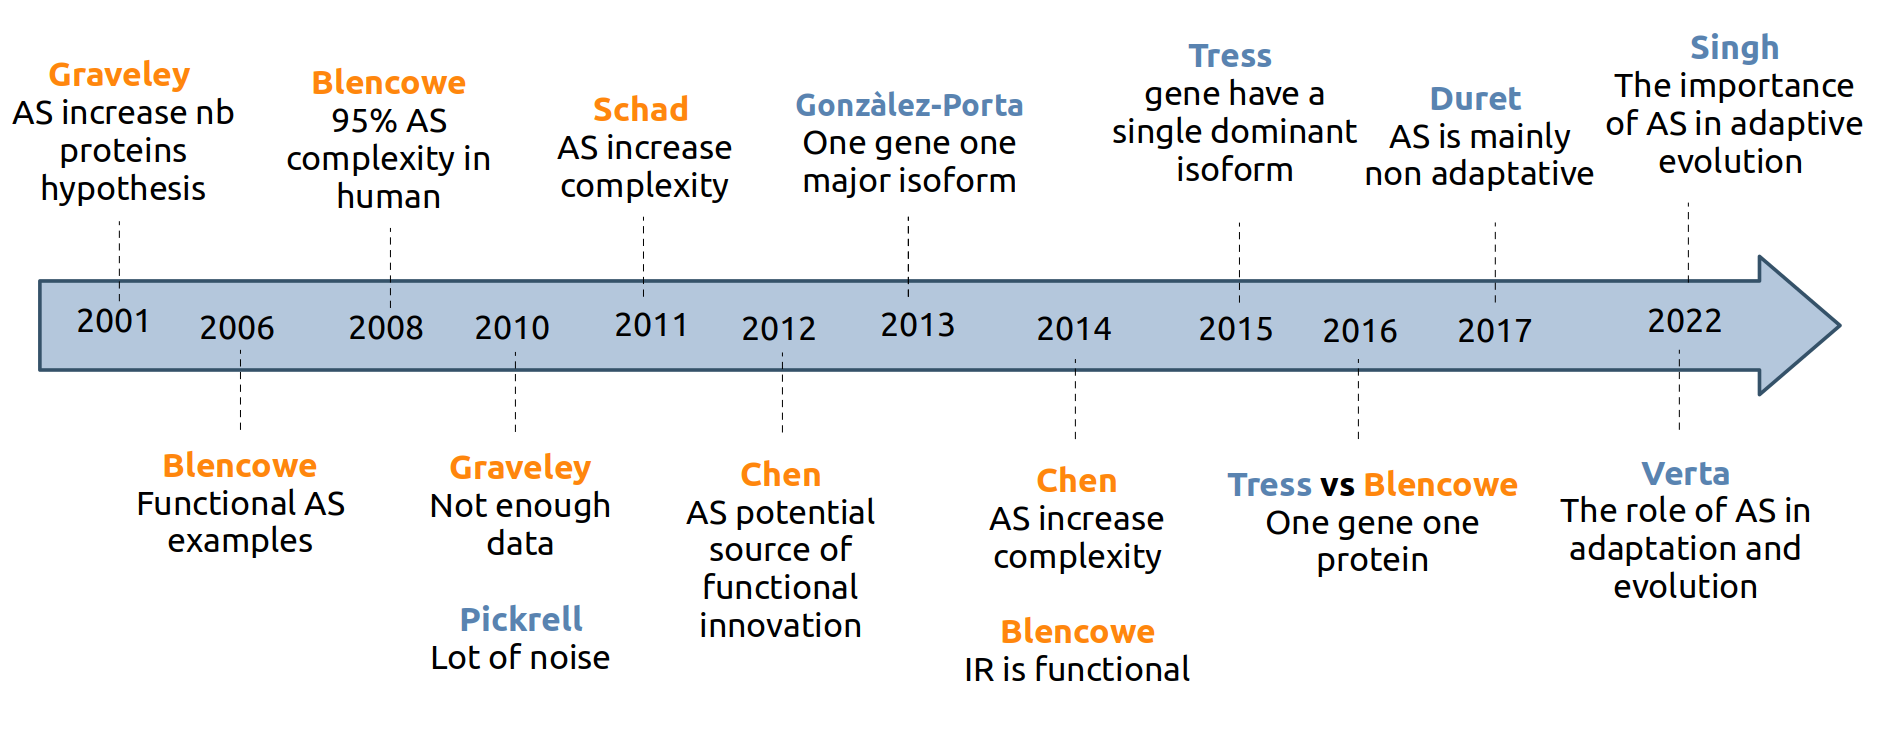
\includegraphics[width=\linewidth]{figures/chronology_as_paper.png}
    \caption[Chronology of the literature on the “raidon d'être” of alternative splicing]{\textbf{Chronology of the literature on the “raidon d'être” of alternative splicing.} Chronology of the main papers taking position in favor of AS primarily increasing proteome diversity (orange) or generating mostly erroneous variants (blue).}
    \label{fig:chronologyaspaper}
\end{figure}

In contemporary literature, the resonance of this far-reaching assertion reverberates, with alternative interpretations in recent publications entitled “the importance of \acrshort{AS} in adaptive evolution"~\citep{singh_importance_2022}, “The role of alternative splicing in adaptation and evolution"~\citep{verta_role_2022}. It is not my intent to discredit this work, but rather, to underscore the necessity of addressing the fundamental question of whether alternative splicing (AS) is predominantly adaptive or non-adaptive. It is essential to clarify that our critique does not stem from an assertion of the prior work's inaccuracy but rather from the paucity of concrete findings pertaining to this specific inquiry. However, it is important to note that numerous studies have probed the functionality of \acrshort{AS}, and the existence of one observation, functional variants, does not negate the possibility of a substantial number of erroneous variants.

In the aforementioned papers, the study~\citet{chen_correcting_2014} is cited to make the assertion that \textit{`A convincing argument for the importance of alternative splicing in organismal evolution was made by~\citet{chen_correcting_2014}'~\citep{singh_importance_2022}}. However, it is prudent to acknowledge that this study may be considered outdated as mentioned earlier. Notably, the authors themselves acknowledge that \textit{`The functional impact of most splice variants on organismal \gls{phenotype} has been the source of extensive debate as it is largely unknown to what extent different alternative isoforms are translated into functional proteins that can alter \gls{phenotype}s and hold adaptive importance'~\citep{singh_importance_2022}}.


\subsection{A fresh perspective through the “drift barrier”}

In order to address the question of whether alternative splicing (\acrshort{AS}) is primarily adaptive or not, we developed a research protocol based on the “drift barrier” hypothesis proposed by~\citet{lynch_frailty_2007} (see `\nameref{geneticdrift}' section).

Population genetics principles posit that the capacity of selection to favor advantageous mutations or eliminate detrimental ones hinges on the strength of selection (\acrshort{s}) relative to the influence of random genetic drift, which is characterized by the effective population size (\acrshort{Ne}). When the selection coefficient is considerably weaker than drift ($|\acrshort{Ne}\acrshort{s}| \ll 1 $), \gls{allele}s behave as if they are effectively neutral. Consequently, random genetic drift imposes an upper limit on selection's ability to impede the fixation of suboptimal \gls{allele}s~\citep{kimura_mutation_1963, ohta_slightly_1973}. This concept, known as the “drift barrier”, as introduced by~\citet{lynch_frailty_2007}, is expected to have repercussions on the efficiency of various cellular processes, including splicing. Therefore, species with lower \acrshort{Ne}~values are anticipated to be more susceptible to splicing errors compared to species with higher \acrshort{Ne}~values.

To assess this hypothesis and analyze the impact of genetic drift on alternative splicing patterns, we calculated \acrshort{AS} rates in 53 metazoan species, utilizing the initial release of our data resource. These species represent a wide spectrum of \acrshort{Ne}~values and were selected based on the availability of high-depth transcriptome sequencing data.

Our research was inspired by the findings of~\citet{braunschweig_widespread_2014} and~\citet{saudemont_fitness_2017}, as well as the earlier hypothesis put forth by~\citet{chen_correcting_2014}. Indeed, under a non-adaptive model, genes expressed at lower levels experience reduced selective pressure, leading to an expectation of greater splicing errors in lowly expressed genes compared to highly expressed ones. We extended this investigation across all the species included in our study to ascertain whether this pattern remains consistent across various species and clades. Finally, we sought to identify functional variant signals, such as the preservation of the reading frame of major isoforms among splicing variants.


\section{Synonymous codons usage among metazoans}

In the early days of deciphering genetic codes, it became evident that the usage of synonymous \gls{codon}s is not uniform; certain synonymous codons are used more frequently than others~\citep{grantham_codon_1980, grantham_codon_1980-1, ikemura_correlation_1981, gouy_codon_1982, sharp_codon_1988, mouchiroud_compositional_1988}. This non-uniform utilization of synonymous codons is observed to exhibit considerable variation among different species~\citep{duret_expression_1999}. Therefore, the second scientific investigation of my thesis is to elucidate the underlying factors contributing to the variability in synonymous codon usage within animal taxa. In particular, I wanted to test whether the selection on synonymous codons usage for optimizing translation depends on random genetic drift intensity.

\subsection{Causes of codon usage variations, a long standing debate}

The utilization of synonymous codons is under the influence of two distinct but non-exclusive processes: non-adaptive and adaptive mechanisms~\citep{bulmer_selection-mutation-drift_1991, duret_trna_2000, duret_evolution_2002, plotkin_synonymous_2011, doherty_translational_2013, parvathy_codon_2022}. 

The non-adaptive model posits that genome-wide mutation patterns and factors such as GC-\gls{biased gene conversion} (\acrshort{gBGC}), which is influenced by recombination rates, play a role in shaping synonymous codon usage~\citep{ikemura_correlation_1981, kanaya_codon_2001, chen_codon_2004, pouyet_recombination_2017}. These processes affect the entire genome and are regrouped under the term of neutral \gls{substitution} patterns (\acrshort{NSP}), whose variations can be observed in non-coding regions.

The adaptive model suggests the existence of optimal synonymous codons for translation, aiming for rapid, high-fidelity translation. This concept is known as \gls{translational selection} and is expected to drive the usage of these optimal codons. One key prediction of this model is that optimal codons should correspond to those decoded by the most abundant tRNA, facilitating accelerated translation~\citep{akashi_synonymous_1994, drummond_mistranslation-induced_2008, hershberg_selection_2008, morris_ribosome_2021}, while minimizing translation errors~\citep{stoletzki_synonymous_2007, kramer_frequency_2007, sun_preferred_2022}. It is worth noting that, in certain cases, such as the folding of protein structures, there may be a rationale for slowing ribosome translation~\citep{yu_codon_2015, liu_code_2020,  weinberg_improved_2016, hussmann_understanding_2015}.

Another key prediction of the adaptive model is that the intensity of \gls{translational selection} should correlate with gene expression, as highly expressed genes require a larger number of ribosomes for their translation. Consequently, the utilization of suboptimal codons in those genes is anticipated to exert a more pronounced influence on the organism's fitness. Consequently, the codon usage of highly expressed genes is expected to better match the tRNA pool. This correlation has been observed in a variety of organisms, including \textit{Drosophila melanogaster}, \textit{Escherichia coli}, and \textit{Caenorhabditis elegans}~\citep{ikemura_correlation_1981, sharp_codon_1988, percudani_restricted_2001, duret_expression_1999, duret_trna_2000}.

However, in vertebrates, \gls{translational selection} in highly expressed genes seems very weak \citep{dos_reis_estimating_2009, doherty_translational_2013}. Indeed, \citet{dos_reis_estimating_2009} showed that the population-scaled selection coefficient estimated on 9 amino acids, is weak in human and mouse, whereas \textit{Drosophila melanogaster} and \textit{Caenorhabditis elegans} have a higher \gls{translational selection}. Also, they pointed out that their estimation might be incorrect because they did not take into account the nucleotide heterogeneity along genomes. Methods for quantifying \gls{translational selection} in these interesting findings may seem circular, because \acrshort{TS} is often estimated by considering codons predominant in highly expressed genes as optimal, to finally quantify their degree of predominance. Thus, \acrshort{TS} estimators are always positive and may, in fact, be overestimated, because the predominance of these codons could be due to variations in mutational biases along the genome.

A long-standing and controversial question involves the examination of human genome, which has not revealed clear indications of \gls{translational selection}. Indeed, there is substantial evidence suggesting that non-adaptive processes significantly influence codon usage bias. Notably, the \acrshort{GC3} content, representing the compositional bias at the third position of codons, reflects synonymous codon usage variations and correlates with genome base composition. This suggests that codon usage is affected by process affecting the entire genome, not only regions subject to \gls{translational selection}~\citep{mouchiroud_compositional_1988, mouchiroud_distribution_1991, kanaya_codon_2001, chen_codon_2004, clay_gc3_2011}.

Nonetheless, the debate regarding the impact of translational selection on the human genome remains highly contested, largely due to variations in non-adaptive processes that are often overlooked in studies. 
As example, several investigations have reported variations in human codon usage across genes expressed in different tissues or cell types ~\citep{vinogradov_dna_2003, plotkin_tissue-specific_2004, gingold_dual_2014}. \citet{gingold_dual_2014} demonstrated significant variations in synonymous codon usage (\acrshort{CU}) among genes associated with cellular proliferation and differentiation. Additionally, they observed that the expression of the \acrshort{tRNA} pool varies across different cell types, each of which expresses specific sets of genes whose coding sequences may be co-adapted with specific pools of \acrshort{tRNA}s. These findings, if valid, suggest a substantial role of translational selection in regulating and determining cell fate.

However, contradictory evidences have been presented suggesting that, despite changes in the tRNA pool between cells, the collective expression of tRNAs with a particular anticodon remains stable throughout development~\citep{schmitt_high-resolution_2014}. Another study showed no covariation between tRNA pool and codon usage in contrasting cells undergoing proliferation and differentiation~\citep{rudolph_codon-driven_2016}. Furthermore,~\citet{pouyet_recombination_2017} presented evidences that meiotic activity determines CU, as differences in CU between sets of genes reflect disparities in meiotic activity linked to recombination and, consequently, genetic \gls{biased gene conversion} (\acrshort{gBGC}). The prevalence of strong \acrshort{gBGC} in mammalian genomes may preclude translational selection from co-adapting the \acrshort{tRNA} pools to the codon demand.

More recently,~\citet{dhindsa_natural_2020} identified distinct gene classes employing specific sets of codons, which they interpreted as indicative of translational selection. It is important to note, however, that they did not consider the role of \acrshort{gBGC} in their study, despite the well-established preference for GC \gls{allele}s due to \acrshort{gBGC} in humans. Because of this, their results led them to conclude that the transition from optimal to non-optimal codons is less favorable compared to the reverse transition. Nevertheless, their study predominantly focuses on GC to AT transitions, which are heavily influenced by \acrshort{gBGC}, and they do not acknowledge this factor in their paper. The debate, therefore, remains unresolved due to the occasional forgetting of non-adaptive models in scientific investigations.


\subsection{Evaluating translational selection intensity and its relation to drift}

In our study, we aim to explore synonymous \gls{codon} usage across animals and determine the causes, whether adaptive or not, underlying these variations. Additionally, we intend to investigate the impact of random genetic drift on \gls{translational selection} (\acrshort{TS}). Indeed, under the “drift barrier” hypothesis, a strong random genetic drift leaves little room for translational selection to operate. 

To provide answers to this long standing debate we propose to systematically analyzed \acrshort{CU} and \acrshort{TS} in metazoans, based on previous approaches on model species. We possess an extensive resource covering a multitude of species, with which we address various research questions. Our protocol is based on the differentiation of genomic regions affected by non-\acrshort{TS} processes, \textit{i.e.} introns, and regions influenced by both non-\acrshort{TS} processes and \acrshort{TS}, \textit{i.e.} exons.

One primary question that we aim to tackle is about the influence of neutral \gls{substitution} patterns (\acrshort{NSP}) on synonymous \gls{codon} usage across species. To do so we aimed at systematically compile intronic data from genes to estimate the neutral \gls{substitution} patterns, considering variables such as the genomic GC content. Concurrently, we intend to collect codon usage patterns within exon sequences.

Using the genes expression obtained from \acrshort{RNA}-seq samples, we can investigate another focal point: the variability in \acrshort{TS} intensity across diverse species. To investigate this, we analyze the extent to which codons promoted by \acrshort{TS} are preferentially utilized in highly expressed genes \citep{ikemura_correlation_1981, ikemura_codon_1985, duret_trna_2000}. First, it is crucial to identify codons that should be favored by translation, specifically those decoded by the most abundant \acrshort{tRNA} molecules. To do so, we propose to systematically quantify the copy numbers of each tRNA gene, a measure highly correlated with \acrshort{tRNA} abundance as demonstrated in previous studies on \textit{Homo sapiens} and \textit{Drosophila melanogaster}~\citep{behrens_high-resolution_2021}. In cases where this data is not readily available, we plan to use tRNAscan-SE for \acrshort{tRNA} annotation~\citep{chan_trnascan-se_2021}.

One final inquiry concerns the exploration of factors contributing to variations in \acrshort{TS} intensity. Within the context of this thesis, we examined factors such as the influence of the “drift barrier” on \acrshort{TS}, hence the effective population size, utilizing four proxies.